This chapter first discusses the experiments carried out in order to both improve the performance, and gain a better understanding, of the sub-components implemented. Experiments such as hyperparameter optimisation and ablation studies including both the two dimensional and three dimensional models are discussed. Once the results are cross-validated, the final results achieved by the optimised models are then presented, interpreted, and compared to results achieved by alternative models. Finally, various aspects of the project are critically evaluated.

\section{Two Dimensional Experimentation}

This section reintroduces the initial results achieved by the ``baseline'' 2D model implemented in Chapter \ref{chap:implementation} and then outlines the experiments carried out in an attempt to improve the performance both qualitatively and quantitatively.

\subsection{Initial Results}

\begin{figure}[!b]
    \begin{subfigure}[b]{0.49\textwidth}
        \centering
        \begin{tikzpicture}[scale=0.9]
            \begin{axis}[
                height=\axisdefaultheight,
                ylabel=\small{Loss},
                xlabel=\small{Epochs},
                grid=major,
                legend pos=north east,
                legend cell align=left,
                legend style={fill=white, fill opacity=0.8, draw=none,text opacity=1}]
                \addplot[blue, mark=x] table [x=xs, y=tl, col sep=comma] {csv/base.csv};
                \addlegendentry{\small{Train Loss}}
                \addplot[magenta, mark=x] table [x=xs, y=vl, col sep=comma] {csv/base.csv};
                \addlegendentry{\small{Val Loss}}
            \end{axis}
        \end{tikzpicture}
        \caption{Loss curve}
    \end{subfigure}
    \hfill
    \begin{subfigure}[b]{0.49\textwidth}
        \centering
        \begin{tikzpicture}[scale=0.9]
            \begin{axis}[
                height=\axisdefaultheight,
                ylabel=\small{Accuracy (\%)},
                xlabel=\small{Epochs},
                grid=major,
                legend pos=south east,
                legend cell align=left,
                legend style={fill=white, fill opacity=0.8, draw=none,text opacity=1}]
                \addplot[blue, mark=x] table [x=xs, y=ta, col sep=comma] {csv/base.csv};
                \addlegendentry{\small{Train Accuracy}}
                \addplot[magenta, mark=x] table [x=xs, y=va, col sep=comma] {csv/base.csv};
                \addlegendentry{\small{Val Accuracy}}
            \end{axis}
        \end{tikzpicture}
        \caption{Loss curve}
    \end{subfigure}
    \caption{The loss and accuracy curves achieved when training the model over 20 epochs using the hyperparameters outlined in Table \ref{tab:initialhyperparams}. It is important to note that although the validation loss begins to increase after epoch 13, the validation accuracy does not begin to decrease. Upon visual inspection of the boundary predictions, it could also be seen that the predictions were qualitatively better when the network was trained for 20 epochs rather than 13. The desirable qualitative features of a prediction are outlined in Figure \ref{fig:goodbad}.}
    \label{fig:basetrainacc}
\end{figure}

\begin{figure}[t]
    \centering
    \begin{subfigure}[t]{0.38\textwidth}
        \centering
        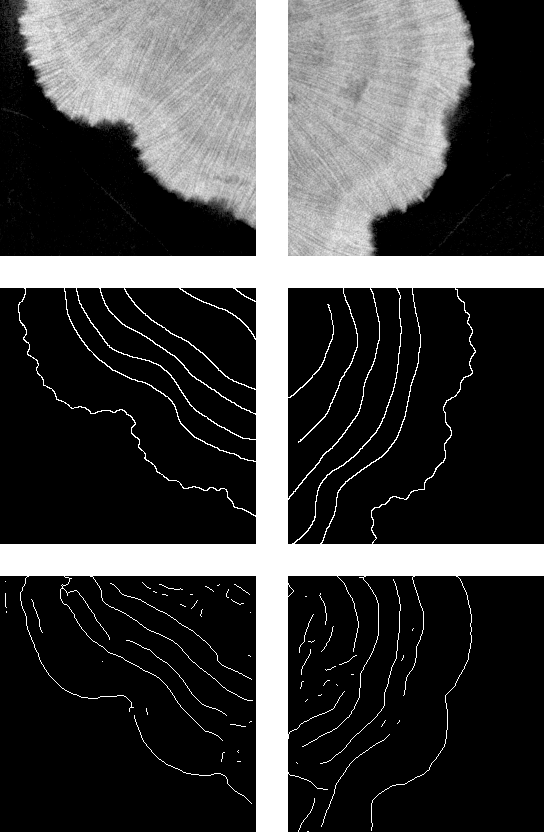
\includegraphics[width=1\textwidth, valign=c]{images/good-initial.png}
        \caption{Higher accuracy: 96.8\% and 96.5\%}
    \end{subfigure}
    ~
    \begin{subfigure}[t]{0.58\textwidth}
        \centering
        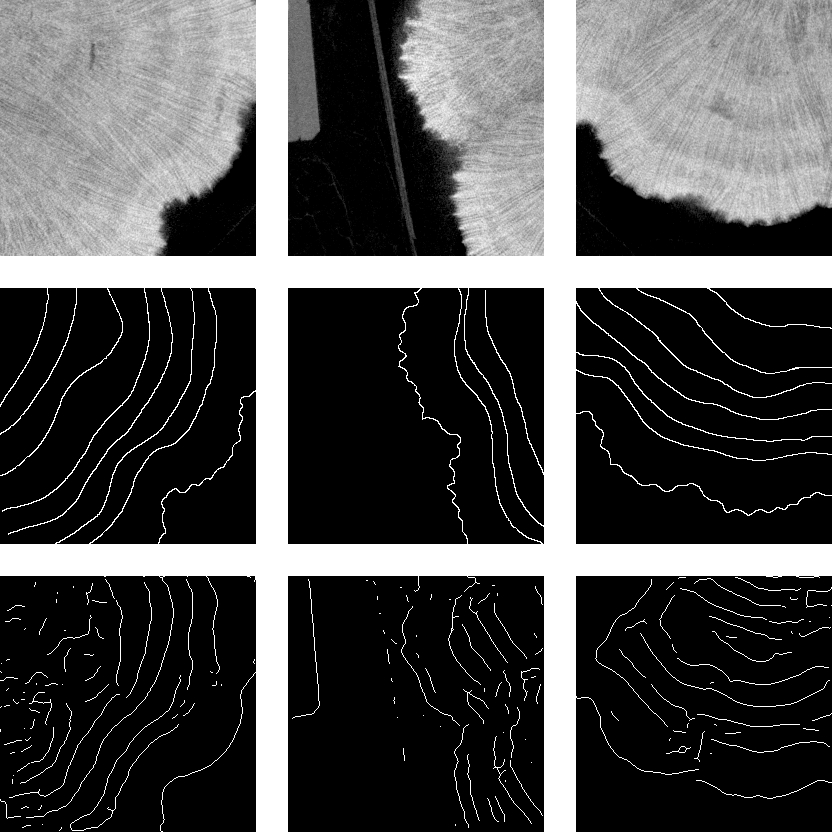
\includegraphics[width=1\textwidth, valign=c]{images/bad-initial.png}
        \caption{Lower accuracy: 92.1\%, 88.4\%, and 91.5\%}
    \end{subfigure}
    \caption{Examples of both high and low quality outputs from the network trained using the initial hyperparameters outlined in Table \ref{tab:initialhyperparams}. The top images are patches from the validation set, the centre images are the corresponding ground truth labels, and the bottom images are the outputs of the network after they have been skeletonized. \textbf{(a)} Examples of high quality predictions. These examples achieved higher accuracies compared to the rest of the samples in the validation set. It can be seen that the boundaries contain comparatively less ``noise'' than the lower quality examples. \textbf{(b)} Examples of low quality predictions. The first example achieves a lower accuracy score due to the noise present in inner section of the coral on the left side of the image. The second example received a particularly low accuracy score due to the accidental classification of the object in the top left of the image as a boundary. This object is the platform that the coral sample is placed on in the CT machine and should perhaps have been cropped from the slices that these patches were produced from. The third example receives a low accuracy due to the accidental misclassification of a boundary perpendicular to the skeleton's surface. As discussed in Chapter \ref{chap:context}, density banding boundaries should be parallel to the coral skeleton surface.}
    \label{fig:goodbad}
\end{figure}

The initial results achieved by the baseline model can be discussed further in order to gain a better understanding of the strengths and weaknesses of the model. The loss and accuracy curves are shown in Figure \ref{fig:basetrainacc} and example boundary predictions of both high and low ``quality'' are shown in Figure \ref{fig:goodbad}. Their quality is assessed both via the accuracy metric achieved and via visual inspection. Looking at Figure \ref{fig:basetrainacc}, it can be see that the accuracy achieved on the validation set is noticeably lower than the accuracy achieved on the training set. This unusual behaviour may be due to the validation set containing ``easier'' examples in which the annual banding is more obvious. Although the performance reported on this validation set may potentially be positively skewed, the final performance achieved by the model will be reported on cross-validated results and so the selection biases that arise from this dataset split should not affect the final reported performance.

\subsection{Hyperparameter optimisation}

As discussed in Chapter \ref{chap:technical}, the performance achieved by deep neural networks is known to depend critically on the identification of a good set of hyperparameters~\cite{hyperparam, goodhyperparam}. In this project, a manual form of grid search was used to discover the optimal set of hyperparameter configurations. In this technique, all hyperparameters are fixed and only a single hyperparameter is varied at a time. Although this may not be the most efficient approach, it enables a better understanding of the model to be gained.

% Due to the time constraints of the project, it would not be possible to perform an exhaustive search of all possible hyperparameter configurations. Thus, the primary aim of this chapter is not to achieve the best performance possible, but instead to evaluate which hyperparameters affect the performance most and reason as to why this is the case.

\subsubsection{Learning Rate}

Of all the hyperparameters relevant to deep learning models, the optimisation of the learning rate often has the biggest impact on the performance of a model~\cite{bengio2012practical}. The selection of a learning rate too large can cause an optimisation algorithm to take a step ``over'' minima causing the loss to inadvertently increase rather than decrease. The selection of a learning rate too small can also hinder performance as the optimisation algorithm may become permanently stuck in a suboptimal local minimum~\cite{goodfellow}.

Since it is usually not possible to calculate an optimal learning rate a priori~\cite{neuralbook}, some form of trial and error is required. A reasonable range of values to experiment with are given by Bengio in~\cite{bengio2012practical} and will be used as the basis of the values experimented with in this section. Bengio suggests an initial learning rate within the range of $10^{-6}$ to $1$.

The accuracies achieved when training the network using various initial learning rates in this range are shown in Figure \ref{fig:lrplot}. It can be seen that the final average accuracy achieved after 20 epochs is similar for all but the 0.00001 value. Although it may look like the accuracy for this learning rate could still improve with further training, the accuracy does not improve further even after 40 epochs. This plateau in the accuracy achieved suggests that the 0.00001 learning rate may be low enough to become stuck in suboptimal local minima.

The training loss achieved by the 0.001 learning rate oscillated at ${\sim}0.5$ for the entire training process, even over multiple training attempts. In comparison, the 0.00005 learning rate achieved a training loss of 0.06 and a validation loss of 0.16. These oscillations are a common sign of a learning rate being too high and stepping ``over'' minima~\cite{bishop1995neural}. Pure black images were output for all samples in both the training and validation set resulting in an accuracy of 0\% being achieved.

Although the both the 0.00005 and 0.0001 learning rates all achieved a similar accuracy of ${\sim}96\%$ after 20 epochs, the 0.00005 value was ultimately chosen for multiple reasons. First, the training and validation accuracy curves are smoother than the curves resulting from higher values, allowing the accuracy to be more reliably used as a stopping criteria for early stopping. Second, when inspecting the results visually, the 0.00005 learning rate results in predictions that are far clearer in the inner areas of the coral skeleton than any other learning rate. Although most of the learning rates were able to produce acceptable predictions nearer to the surface of the coral, only the 0.00005 learning rate was able to produce acceptable predictions in these inner areas. An example of a patch that benefited from the 0.00005 learning rate is shown in Figure \ref{fig:lrdiff}.

\begin{figure}[!t]
    \centering
    \begin{subfigure}[t]{0.32\textwidth}
        \centering
        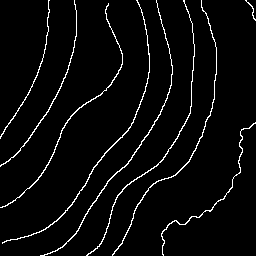
\includegraphics[width=1\textwidth, valign=c]{images/lr-comparison.png}
        \caption{Ground truth boundaries}
    \end{subfigure}
    ~
    \begin{subfigure}[t]{0.32\textwidth}
        \centering
        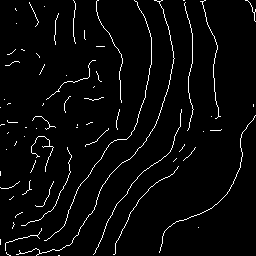
\includegraphics[width=1\textwidth, valign=c]{images/1e4-example.png}
        \caption{$\eta=0.0001$ prediction}
    \end{subfigure}
    ~
    \begin{subfigure}[t]{0.32\textwidth}
        \centering
        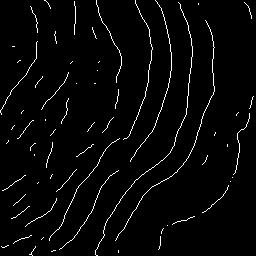
\includegraphics[width=1\textwidth, valign=c]{images/5e5-example.png}
        \caption{$\eta=0.00005$ prediction}
    \end{subfigure}
    \caption{An example of a patch that benefits from the a learning rate $\eta$ of 0.00005. The $\eta=0.0001$ prediction achieved an accuracy of 92.1\% whereas the $\eta=0.00005$ prediction achieved an accuracy of 95.5\%. The 0.0001 prediction achieves a lower accuracy score due to the noise present in inner section of the coral on the left side of the image. The 0.00005 prediction has more realistic predictions in this area of the image with all boundaries seeming close to parallel to the growth surface of the skeleton.}
    \label{fig:lrdiff}
\end{figure}

\begin{figure}[!t]
    \begin{subfigure}[b]{0.49\textwidth}
        \centering
        \begin{tikzpicture}[scale=0.9]
            \begin{axis}[
                height=\axisdefaultheight,
                ylabel=\small{Accuracy (\%)},
                xlabel=\small{Epochs},
                grid=major,
                legend pos=south east,
                legend cell align=left,
                legend style={fill=white, fill opacity=0.8, draw=none,text opacity=1}]
                \addplot[magenta, mark=x] table [x=xs, y=lr00001_vacc, col sep=comma] {csv/lr.csv};
                \addlegendentry{\small{$\eta=0.00001$}}
                \addplot[darkgray, mark=x] table [x=xs, y=lr00005_vacc, col sep=comma] {csv/lr.csv};
                \addlegendentry{\small{$\eta=0.00005$}}
                \addplot[blue, mark=x] table [x=xs, y=lr0001_vacc, col sep=comma] {csv/lr.csv};
                \addlegendentry{\small{$\eta=0.0001$}}
                \addplot[orange, mark=x] table [x=xs, y=lr0005_vacc, col sep=comma] {csv/lr.csv};
                \addlegendentry{\small{$\eta=0.0005$}}
            \end{axis}
        \end{tikzpicture}
        \caption{Varying learning rate}
        \label{fig:lrplot}
    \end{subfigure}
    \hfill
    \begin{subfigure}[b]{0.49\textwidth}
        \centering
        \begin{tikzpicture}[scale=0.9]
            \begin{axis}[
                height=\axisdefaultheight,
                ylabel=\small{Accuracy (\%)},
                xlabel=\small{Epochs},
                grid=major,
                legend pos=south east,
                legend cell align=left,
                legend style={fill=white, fill opacity=0.8, draw=none,text opacity=1}]
                \addplot[magenta, mark=x] table [x=xs, y=bs1_vacc, col sep=comma] {csv/batch.csv};
                \addlegendentry{\small{$batch=1$}}
                \addplot[darkgray, mark=x] table [x=xs, y=bs2_vacc, col sep=comma] {csv/batch.csv};
                \addlegendentry{\small{$batch=2$}}
                \addplot[blue, mark=x] table [x=xs, y=bs4_vacc, col sep=comma] {csv/batch.csv};
                \addlegendentry{\small{$batch=4$}}
                \addplot[teal, mark=x] table [x=xs, y=bs8_vacc, col sep=comma] {csv/batch.csv};
                \addlegendentry{\small{$batch=8$}}
                \addplot[orange, mark=x] table [x=xs, y=bs16_vacc, col sep=comma] {csv/batch.csv};
                \addlegendentry{\small{$batch=16$}}
            \end{axis}
        \end{tikzpicture}
        \caption{Varying batch size}
        \label{fig:bsplot}
    \end{subfigure}
    \caption{The accuracies achieved on the validation set using various hyperparameter values. A TensorBoard smoothing value of 0.3 was used. \textbf{(a)} The accuracies achieved when training the network using various initial learning rate values $\eta$. Apart from the learning rate, the same hyperparameters used to achieve the initial results (outlined in Table \ref{tab:initialhyperparams}) were used once again. \textbf{(b)} The accuracies achieved when training the network using various batch sizes. Apart from a learning rate of 0.00005 being used, the hyperparameters outlined in Table \ref{tab:initialhyperparams} were used once again.}
\end{figure}

\subsubsection{Batch Size}

The next parameter experimented with was the batch size. Ranging from a size of one up to a few hundreds in some applications~\cite{bengio2012practical}, the batch size not only affects the performance achieved by a network, but can also affect training times significantly.

Small batches with sizes equal to powers of two were experimented with. The accuracies achieved when training using these various batch sizes are shown in Figure \ref{fig:bsplot}. Looking at Figure \ref{fig:bsplot}, it can already be seen that as the batch size increases, the accuracy achieved by the model decreases (with the exception of a batch size of one). Batch sizes greater than 16 were also experimented with but the accuracy achieved only continued to decrease. It may seem that the accuracy achieved still increase further given more training epochs, however even after 40 epochs the network trained with $batch=8$ only achieved an accuracy of 91\% compared to the accuracy of 95\% achieved when $batch=2$. Note that in order to ensure that the model was exposed to the same number of samples per epoch, with each increase in batch size, the \texttt{steps-per-epoch} argument of the \texttt{fit} method was also decreased. For example, if the batch size was doubled, the \texttt{steps-per-epoch} was halved. This is due to the \texttt{steps-per-epoch} argument specifying how many batches compose an epoch, rather than how many samples compose an epoch.

In practice, it has often been observed that larger batch sizes result in lower accuracy being achieved in deep learning models~\cite{keskar2016large, smallbatch, largebatch}. Keskar et al. propose that this decrease in performance may be attributed to larger batch sizes converging to ``sharp'' minima~\cite{keskar2016large}. Whilst a ``flatter'' minimum can be described with low precision, a sharp minimum requires high precision. Keskar et al. cite the minimum description length (MDL) theory, which states that statistical models that require fewer bits to describe generalise better~\cite{rissanen}, and argue that since flat minisers can be specified with lower precision, they tend to have better generalisation performance. Note that the accuracy achieved on the validation set is a measure of how well the network generalises, since the network has not yet been trained on any slices present in the validation set.

Ultimately, a batch size of two was decided upon as the network trained with this size achieved the highest training and validation accuracy. Although a batch size of 16 provided a ${\sim}1.4$ times speed up in the training process, the model still trains in under 20 minutes\footnote{When trained using an Nvidia P100 ``Pascal'' GPU.} when using a batch size of two. For now, the improved performance provided by a smaller batch size outweighs the benefits provided by the training time saved when using larger sizes. If vast amounts of labelled data were available, a larger batch size would likely be necessary to keep training times reasonable.

\subsubsection{Optimisation Algorithms}

This section discusses experimention carried out with the stochastic gradient descent (SGD) optimisation algorithm. SGD was used successfully to train the original U-Net architecture to perform semantic segmentation on 2D greyscale biomedical data~\cite{ronneberger2015u} and so is a reasonable alternative choice to the Adam optimiser used so far.

The Keras implementation of Stochastic Gradient Descent (SGD) was experimented with. Learning rates of 0.00005, 0.0001, 0.0005, and 0.001 were all experimented with but none yielded acceptable results. Momentum 0.5 and 0.9 still not acceptable results. Maybe show the image output for all SGD implementations? Explain that a nearly constant accuracy of ... was achieved. (just use the last acc value). Tried momentum 0.5 and 0.9 with learning rates 0.001 and 0.01 and still no good results. Tried learning rates from 0.00005 all the way to 0.01 with and without momentum and nothing worked. larger learning rates output black images, lower all output this image:.

Tried SGD with 0.00005, 0.0001, 0.0005, no good results. maybe example output image? maybe the momentum of adam was very important? loss stuck at 0.16 and val loss never came below 0.3. Very similar results for adam with epsilon=1 and epsilon=? maybe suggests that the epsilon (maybe explain what adam say epsilon does?) is very important for the performance of adam?

Maybe mention the momentum weight update rule used in Keras?

\subsubsection{Loss Functions}

\begin{figure}[!t]
    \includegraphics[width=\textwidth, height=0.6\textwidth]{example-image-b}
    \caption{Focal loss examples vs cross-entropy loss examples.}
    \label{fig:lossfunctiondiff}
\end{figure}

As outlined in Chapter \ref{chap:implementation}, the labelling technique used gives rise to a severe class imbalance. On average, ${\sim}$98\% of a labelled patch is black---part of the ``not part of a boundary'' class. As a result, a model that learned to output a pure black image would achieve a low loss value for ${\sim}$98\% of the image. Although this has proved to be a problem when assessing the accuracy of the model, the effects of this class imbalance on the network's ability to learn are not yet obvious. This section outlines the experiments carried out involving the Focal Loss function designed specifically to address the class imbalance problem.

% Proposed by Lin et al. in 2018, the Focal Loss~\cite{focalloss} is designed to address the ``class imbalance'' problem. In a typical classification problem, class imbalance occurs when one class contains significantly fewer samples than the other classes. Lin et al. highlight the fact that when using the cross-entropy loss function, even samples that are well-classified incur a loss with ``non-trivial'' magnitude. When summed over large numbers of samples from the easily classified majority class, these small loss values can overwhelm the loss resulting from the minority class samples~\cite{focalloss}. As highlighted in Section \ref{sec:challenges}, the boundary extraction task inherently contains a severe class imbalance; the focal loss function could be used to reduce the effects of the class imbalance on the performance of the networks used throughout the project.

% There are two major issues that arise when using a standard per-pixel accuracy metric to quantify the performance achieved in this task. The first issue stems from the severe class imbalance present in the labels. On average, ${\sim}$98\% of a labelled patch is black---part of the ``not part of a boundary'' class. As a result, a model that learned to output a pure black image would achieve an average accuracy of 98\%.

% In an attempt to address this problem, the focal loss introduces two new parameters: a weighting factor $\alpha \in [0, 1]$ and a ``focusing'' parameter $\gamma \geq 0$.
% The binary focal loss is then defined as:

% \begin{equation}
%     \text{FL}(p, y) = 
%     \begin{cases}
%         -\alpha(1 - p)^{\gamma} \log (p) & \text{if } y = 1\\
%         (1 - \alpha)p^{\gamma} \log (1 - p) & \text{otherwise}
%     \end{cases}
% \end{equation}

% where $y \in \{+1, -1\}$ is the actual value (the ground-truth), and $p \in [0, 1]$ is the model's estimated probability for the class with label $y = 1$. The weighting factor increases the loss produced by the misclassification of minority class samples whilst the focusing factor ``reduces the contribution from easy examples and extends the range in which an example receives low loss''~\cite{focalloss}. When $\gamma = 0$ and $\alpha = 1$, the focal loss is equivalent to the cross-entropy loss. The contribution of the $\gamma$ value to the loss produced can be seen in Figure \ref{fig:focal}.

Look at the alpha and gamma values of focal loss? play around with them a little. look at the table in the original paper that says when you should use what.

At the end of this section, resummarise the configuration of chosen params now in Table \ref{tab:hyperparams1}.

\begin{table}[t]
    \centering
    \caption{A summary of the initial hyperparameter settings used.}
    \begin{tabular}{@{}ll@{}}
    \toprule
    Hyperparameter   & Setting      \\ \midrule
    Architecture     & 2D U-Net   \\
    Optimiser & Adam \\
    Learning rate & 0.00005 \\
    Loss function & Cross-entropy \\
    Epochs & 20 \\
    Steps per epoch & 500 \\
    Batch size & 2 \\ \bottomrule
    \end{tabular}
    \label{tab:hyperparams1}
\end{table}

\subsubsection{Dropout}

% Another technique often used to reduce overfitting is dropout. The use of dropout as a regularization technique when training neural networks was first popularised by Srivastava et al.~\cite{dropout} in 2014. Throughout the training process, subsets of randomly selected neurons (and their connections) are ``dropped''. Only the resulting reduced network is then trained on a particular training sample. A subset of dropped neurons will only remain dropped whilst processing a single training sample; the dropped neurons will then be added back to the network and a different subset of neurons will be dropped when processing the next training sample. The choice of which subset of neurons to drop for each training sample is random. 

% Dropout reduces overfitting by preventing neurons from ``co-adapting'' too much~\cite{dropout}. Co-adaptation between neurons refers to the phenomenon when one neuron relies too heavily on the input from another neuron. If one neuron relies too heavily on the input of another neuron, the receiving neuron's performance in producing an activation that would be beneficial to the performance of the network may be hindered by the one ``bad'' input---even if the inputs from all other incoming neurons were ``good''. In this case, the terms good and bad are used to describe whether or not an input helped in contributing to the the beneficial activation value calculated via backpropagation.

REMEMBER TO TRY AND UNDERSTAND WHY WHAT EVER HAPPENS IS THE CASE AND BACK IT UP ALL THROUGHOUT

vary from 0.1 to 0.9? same with spatial

\subsubsection{Spatial Dropout}

Need to talk about dropout? maybe only mention it in evaluation?
Spatial drop out better for fully conv? \url{https://arxiv.org/pdf/1411.4280.pdf}

% From Keras docs I think
% This version performs the same function as Dropout, however it drops
% entire 2D feature maps instead of individual elements. If adjacent pixels
% within feature maps are strongly correlated (as is normally the case in
% early convolution layers) then regular dropout will not regularize the
% activations and will otherwise just result in an effective learning rate
% decrease. In this case, SpatialDropout2D will help promote independence
% between feature maps and should be used instead.

\subsubsection{Kernel Sizes}

\subsubsection{L2 Regularization}

\subsection{Resolution}

In order to gain a better understanding of the U-Net architecture, the resolutions

\subsection{Augmentation}
\label{sec:evalaugmentation}

\subsubsection{No Augmentation}

I said in Chapter \ref{chap:implementation} that augmentation was very important.

\subsubsection{Augmentation Ranges}

\subsection{Ablation Studies}

comparison of convtranspose to upsample and then conv.

remove the relu at the end of the implementation?

Maybe visualise ablations with a graph showing each ablation with accuracy achieved or something? like in that paper. or a table?

\begin{figure}[!t]
    \centering
    \begin{tikzpicture}[scale=0.9]
        \begin{axis}[
            height=\axisdefaultheight,
            width=0.6\textwidth,
            ylabel=\small{Accuracy (\%)},
            xlabel=\small{Epochs},
            grid=major,
            legend pos=south east,
            legend cell align=left,
            legend style={fill=white, fill opacity=0.8, draw=none,text opacity=1}]
            \addplot[magenta, mark=x] table [x=xs, y=lr00001_vacc, col sep=comma] {csv/lr.csv};
            \addlegendentry{\small{$\eta=0.00001$}}
            \addplot[darkgray, mark=x] table [x=xs, y=lr00005_vacc, col sep=comma] {csv/lr.csv};
            \addlegendentry{\small{$\eta=0.00005$}}
            \addplot[blue, mark=x] table [x=xs, y=lr0001_vacc, col sep=comma] {csv/lr.csv};
            \addlegendentry{\small{$\eta=0.0001$}}
            \addplot[orange, mark=x] table [x=xs, y=lr0005_vacc, col sep=comma] {csv/lr.csv};
            \addlegendentry{\small{$\eta=0.0005$}}
        \end{axis}
    \end{tikzpicture}
    \caption{Ablation}
    \label{fig:ablationplot}
\end{figure}

\section{Three Dimensional Experimentation}

\subsection{Hyperparameter optimisation}

Due to the time constraints of the project, far fewer hyperparameters were optimised for the three dimensional architectures.

Briefly mention that various learning rates and batch sizes were experimented with but none produced better results (unless then do?) and the new optimal hyperparameters for the 2D arch were used.

\subsection{Augmentation}

\subsection{Alternative Modified Architectures}

Varying numbers of output channels in Conv3D layers as you said youd experiment with this.

\subsection{Fully Three Dimensional Architecture}

\subsubsection{Data}

Lack of data. Was not consistently labelled. Show adjacent slices. Proves how hard it is to label images.

\section{Cross-validation}
\label{sec:evalcrossval}

As outlined in Chapter \ref{chap:technical}, cross-validation is designed to give a comprehensive measure of a model's performance throughout the entire dataset, rather than just a particular subset. Cross-validation techniques reduce the effects of selection bias on the reported performance. Since the slices composing the test set and the slices composing the training set were extracted from different samples, some form of selection bias is inevitable and the performance achieved on the current test set does not necessarily represent the performance that would be achieved on the entire dataset.

\subsection{Train/test Splits}

In order to perform cross-validation, the dataset must be split into multiple training and testing sets---``train/test'' splits. Similarly to how the dataset was split in Chapter \ref{chap:implementation}, the

\section{Final Results}

\begin{figure}[!p]
    \centering
    \includegraphics[width=\textwidth, height=1.45\textwidth]{example-image-b}
    \caption{A full page of final results achieved.}
    \label{fig:finalresults}
\end{figure}

\section{Comparisons with Other Architectures}

Compare SegNet, U-Net, pix2pix. Maybe find somewhere to put in the pix2pix generation for fun? If not don't worry. Do mention pix2pix using different backbones or whatever its called and why you think it didnt perform well.

\subsection{SegNet}

\subsection{pix2pix}



\section{Critical Evaluation}

\subsection{Boundary Extraction}

\subsubsection{Labelling}

Could have chosen the thick style as this would get rid of the class imbalance and would allow for a normal accuracy metric etc. Mention again how hard it is to be consistent.

\subsubsection{Lack of Data}

very hard for a non expert to label.

\subsection{Accuracy Metric}

Can't tell which boundary it should be looking for. a completely white image would produce 100\% accuracy but the skeletonization makes the amount of white pixels low.

Maybe show concrete examples of where it falls down? images shifted to the right so that one boundary is roughly where another should be? images that have many white lines that are even perpendicular to the right labels should still produce a pretty low score?

Show image produced by SGD. completely wrong but still gets 60\% due to the white part in the bottom left of the image. this might be fixed now that we use a max of 90?

visual inspection is still needed take for example the learning rate plots, they all achieve accuracies within a percentage of each other but some are clearly worse than others?

\subsection{Calcification Rate Estimation}

\section{Comparisons with Existing Techniques}

Erica sent a paper a while ago that used a computer program to calculate the calcification rate  \url{https://www.geosociety.org/datarepository/2015/2015015.pdf} check the email from her with subject DeCarlo Paper

% {\bf A topic-specific chapter, of roughly $15$ pages} 
% \vspace{1cm} 

% \noindent
% This chapter is intended to evaluate what you did.  The content is highly 
% topic-specific, but for many projects will have flavours of the following:

% \begin{enumerate}
% \item functional  testing, including analysis and explanation of failure 
%       cases,
% \item behavioural testing, often including analysis of any results that 
%       draw some form of conclusion wrt. the aims and objectives,
%       and
% \item evaluation of options and decisions within the project, and/or a
%       comparison with alternatives.
% \end{enumerate}

% \noindent
% This chapter often acts to differentiate project quality: even if the work
% completed is of a high technical quality, critical yet objective evaluation 
% and comparison of the outcomes is crucial.  In essence, the reader wants to
% learn something, so the worst examples amount to simple statements of fact 
% (e.g., ``graph X shows the result is Y''); the best examples are analytical 
% and exploratory (e.g., ``graph X shows the result is Y, which means Z; this 
% contradicts [1], which may be because I use a different assumption'').  As 
% such, both positive {\em and} negative outcomes are valid {\em if} presented 
% in a suitable manner.